% !TeX spellcheck = es_ES
\documentclass[12pt]{article}

% --- PAQUETES ---
\usepackage[utf8]{inputenc}
\usepackage[spanish,es-nodecimaldot]{babel}
\usepackage{graphicx}
\usepackage[margin=2.5cm]{geometry}
\usepackage{float}
\usepackage{amsmath}
\usepackage{amsfonts}

% --- COMANDOS PERSONALIZADOS ---
\newcommand{\hrules}{\rule{\linewidth}{0.5mm}}

\begin{document}
	
	\begin{titlepage}
		\centering
		
		% Cabecera institucional
		\begin{minipage}[c]{0.2\textwidth}
			
\includegraphics[width=\linewidth]{logo_ipn.png}
		\end{minipage}%
		\hfill
		\begin{minipage}[c]{0.55\textwidth}
			\centering
			{\scshape\Large Instituto Politécnico Nacional}\\[0.3cm]
			{\scshape\large Escuela Superior de Cómputo}
		\end{minipage}%
		\hfill
		\begin{minipage}[c]{0.2\textwidth}
			\raggedleft
			
\includegraphics[width=\linewidth]{logo_escom.png}
		\end{minipage}
		
		\vspace{1.5cm}
		
		{\large\textbf{Ingeniería en Inteligencia Artificial}}\\[1.5cm]
		
		{\Large\textbf{Reconocimiento de voz}}\\[2cm]
		
		\hrules
		\vspace{0.4cm}
		{\huge\bfseries Práctica 1: Representación del habla}\\[0.4cm]
		\hrules
		\vspace{2.5cm}
		
		% Información personal
		\begin{minipage}{0.8\textwidth}
			\large
			\textbf{Profesor:}\\
			Enrique Alfonso Carmona García\\[1cm]
			
			\textbf{Alumno:}\\
			Velázquez Arrieta Eduardo Uriel
		\end{minipage}
		
		\vfill
		
		{\large Fecha de entrega: 25 de septiembre de 2026}
		
	\end{titlepage}
	
	\newpage
	\tableofcontents % Índice de contenido
	\vspace{1cm}
	\listoffigures   % Índice de imágenes
	\newpage
	
	% Aquí inicia el contenido de tu práctica
	
	\section{Introducción}
	El procesamiento y reconocimiento automático del habla requiere transformar la señal acústica continua unidimensional en una representación compacta y representativa que capture las características fonéticas esenciales del tracto vocal humano, descartando variaciones irrelevantes como el ruido de fondo o peculiaridades del canal de transmisión. Entre las técnicas más consolidadas en este ámbito destacan los Coeficientes Cepstrales en las Frecuencias de Mel (\textit{Mel-Frequency Cepstral Coefficients}, MFCC), los cuales modelan la percepción auditiva no lineal del oído humano mediante un banco de filtros espaciados triangularmente en la escala Mel y una descorrelación espectral mediante la Transformada de Coseno Discreta (DCT).
	
	El objetivo principal de esta práctica es implementar y contrastar rigurosamente dos enfoques metodológicos para la extracción de coeficientes MFCC a partir de una misma señal de voz:
	\begin{enumerate}
		\item \textbf{Implementación manual paso a paso:} Diseñar y computar la cadena completa de procesamiento digital de señales sin recurrir a funciones de alto nivel preconstruidas para MFCC, abarcando las etapas de preénfasis, segmentación en tramas (\textit{framing}), ventaneo temporal (Hamming), cálculo del espectro de potencia mediante la Transformada Rápida de Fourier (FFT), integración a través de un banco de filtros Mel, compresión logarítmica y la aplicación final de la DCT-II.
		\item \textbf{Implementación estándar mediante biblioteca:} Extraer las características acústicas empleando la función nativa \texttt{librosa.feature.mfcc()} bajo sus configuraciones predeterminadas.
	\end{enumerate}
	
	Para el desarrollo experimental se emplea el lenguaje de programación \textbf{Python}, apoyado en bibliotecas científicas fundamentales como \textbf{NumPy} y \textbf{SciPy} para la formulación vectorial y transformadas matemáticas de la implementación manual, \textbf{Matplotlib} para la generación y renderizado comparativo de espectrogramas y matrices cepstrales, y la librería especializada \textbf{Librosa} junto con \textbf{SoundFile} para la decodificación, manipulación acústica y cómputo de referencia. Asimismo, se integrará un conjunto de datos propio consistente en grabaciones de voz estructuradas a nivel de palabra aislada (\textit{«Casa»}) y habla continua (\textit{«La casa es grande»}).
	
	Como resultado de esta práctica, se espera obtener una reconstrucción visual fidedigna de las matrices de coeficientes cepstrales para ambas señales analizadas, así como cuantificar y justificar analíticamente las posibles discrepancias numéricas y dimensionales observadas entre ambos métodos. Dichas variaciones permitirán discutir en profundidad la influencia de hiperparámetros críticos del procesamiento en tiempo-frecuencia, tales como el tipo de relleno (\textit{padding}), la normalización de área en los filtros Mel, las convenciones en el cálculo de la DCT ortogonal y el solapamiento de las ventanas temporales.
	
\section{Desarrollo}

\subsection{Dataset}
Para la experimentación se conformó un conjunto de datos acústicos compuesto por dos grabaciones de voz en formato digital (\texttt{.mp3}), registradas en un entorno controlado:
\begin{itemize}
	\item \textbf{Audio 1:} Emisión a nivel de palabra aislada correspondiente a la frase \textit{«Casa»}, con una duración aproximada de $1.95\,\text{s}$.
	\item \textbf{Audio 2:} Emisión de habla continua correspondiente a la frase \textit{«La casa es grande»}, con una duración aproximada de $1.85\,\text{s}$.
\end{itemize}
Ambos archivos fueron leídos preservando su frecuencia de muestreo nativa (\texttt{sr=None}) mediante la función \texttt{librosa.load}, la cual normaliza de manera predeterminada la amplitud de la señal al intervalo de punto flotante $[-1.0, 1.0]$.

\subsection{Obtención de los coeficientes MFCC de manera manual}
El algoritmo implementado en la función \texttt{compute\_mfcc} reproduce paso a paso la cadena clásica de procesamiento digital de señales acústicas:

\begin{enumerate}
	\item \textbf{Preénfasis:} Se aplica un filtro FIR paso altas de primer orden expresado como:
	\begin{equation}
		y[n] = x[n] - \alpha x[n-1], \quad \text{con } \alpha = 0.97
	\end{equation}
	En el código se implementa vectorialmente con:
	\begin{verbatim}
		audio = np.append(audio[0], audio[1:] - 0.97 * audio[:-1])
	\end{verbatim}
	Su objetivo es compensar la caída espectral natural de la voz humana (aproximadamente $-6\,\text{dB}$ por octava debido a la radiación labial) y amplificar las altas frecuencias.
	
	\item \textbf{Segmentación en tramas (\textit{Framing}) y Enventanado (\textit{Windowing}):} Las señales de habla son cuasiestacionarias en intervalos de $20$ a $30\,\text{ms}$. Se define una longitud de ventana de $25\,\text{ms}$ (\texttt{win\_length = int(round(0.025 * sample\_rate))}) y un paso de avance (\textit{hop}) de $10\,\text{ms}$ (\texttt{hop\_length = int(round(0.010 * sample\_rate))}). La extracción eficiente de tramas sin copias redundantes de memoria se realiza con \texttt{np.lib.stride\_tricks.as\_strided}. Posteriormente, a cada trama se le aplica una ventana de Hamming simétrica:
	\begin{equation}
		w[n] = 0.54 - 0.46 \cos\left(\frac{2\pi n}{N-1}\right)
	\end{equation}
	implementada mediante \texttt{frames *= np.hamming(win\_length)}, reduciendo así las discontinuidades en los bordes y el fenómeno de fuga espectral (\textit{spectral leakage}).
	
	\item \textbf{Transformada Rápida de Fourier (FFT) y Espectro de Potencia:} Se calcula la Transformada Discreta de Fourier para señales reales con longitud $N_{\text{FFT}} = 512$ (\texttt{np.fft.rfft(frames, n=fft\_length)}). A partir de la magnitud compleja, se estima el espectro de potencia normalizado:
	\begin{equation}
		P(k) = \frac{1}{N_{\text{FFT}}} |X(k)|^2
	\end{equation}
	reflejado en el código como \texttt{power\_spectrum = (1.0 / fft\_length) * (mag\_frames ** 2)}.
	
	\item \textbf{Banco de Filtros Mel:} Se simula la percepción frecuencial no lineal coclear mediante $M = 40$ filtros triangulares solapados linealmente espaciados en la escala Mel:
	\begin{equation}
		m = 2595 \log_{10}\left(1 + \frac{f}{700}\right) \iff f = 700 \left(10^{m / 2595} - 1\right)
	\end{equation}
	Los centros de corte se mapean a los índices de frecuencia (\textit{bins}) de la FFT, generando la matriz \texttt{fb} de dimensiones $(40, 257)$.
	
	\item \textbf{Energía de Filtro y Compresión Logarítmica:} Se proyecta el espectro de potencia sobre el banco Mel mediante un producto punto (\texttt{np.dot(power\_spectrum, fb.T)}). Para evitar indeterminaciones matemáticas por ceros o valores negativos, se acota inferiormente con el épsilon de máquina (\texttt{np.finfo(float).eps}) y se aplica el logaritmo natural:
	\begin{equation}
		S_{\text{log}}[m] = \ln(S[m])
	\end{equation}
	
	\item \textbf{Transformada de Coseno Discreta (DCT):} Se aplica la DCT Tipo II ortonormalizada (\texttt{norm='ortho'}) sobre el eje frecuencial logarítmico para descorrelacionar las componentes energéticas, seleccionando los primeros 13 coeficientes (\texttt{num\_ceps=13}):
	\begin{equation}
		c[n] = \sum_{m=0}^{M-1} S_{\text{log}}[m] \cos\left[\frac{\pi n}{M}\left(m + \frac{1}{2}\right)\right]
	\end{equation}
	
	\item \textbf{Filtrado Cepstral (\textit{Sinusoidal Liftering}):} Para atenuar la susceptibilidad al ruido en coeficientes superiores y balancear la escala dinámica, se aplica una ventana sinusoidal de realce con factor $L = 22$:
	\begin{equation}
		w_c[n] = 1 + \frac{L}{2}\sin\left(\frac{\pi n}{L}\right)
	\end{equation}
\end{enumerate}

\subsection{Obtención de los coeficientes MFCC con librosa}
En la implementación estándar se utilizó la función de alto nivel \texttt{librosa.feature.mfcc(y=y, sr=sr, n\_mfcc=20)}. Las características internas predeterminadas de Librosa conllevan diferencias de diseño fundamentales:
\begin{itemize}
	\item \textbf{Transformada de Tiempo Corto (STFT):} Librosa no aplica preénfasis por defecto. Utiliza una ventana Hann centrada con relleno reflectivo (\textit{centered padding}), con $n_{\text{fft}} = 2048$ y $hop\_length = 512$ muestras.
	\item \textbf{Banco Mel y Escala:} Emplea de manera nativa la formulación Mel de Slaney (con espaciado lineal por debajo de $1\,\text{kHz}$ y logarítmico por encima) y aplica normalización de área unitaria en cada triángulo (\textit{area normalization}).
	\item \textbf{Compresión en Decibelios:} Convierte la potencia acumulada a decibelios en referencia al valor pico (\texttt{power\_to\_db}) en lugar de usar un simple logaritmo neperiano natural.
	\item \textbf{Dimensionalidad:} Por defecto calcula $20$ coeficientes cepstrales y no aplica \textit{liftering} sinusoidal.
\end{itemize}

\subsection{Comparación del primer audio (Audio 1: «Casa»)}
En la Figura~\ref{fig:audio1_comp} se muestra el contraste entre ambas representaciones para el Audio 1.

\begin{figure}[H]
	\centering
	\begin{minipage}{0.48\textwidth}
		\centering
		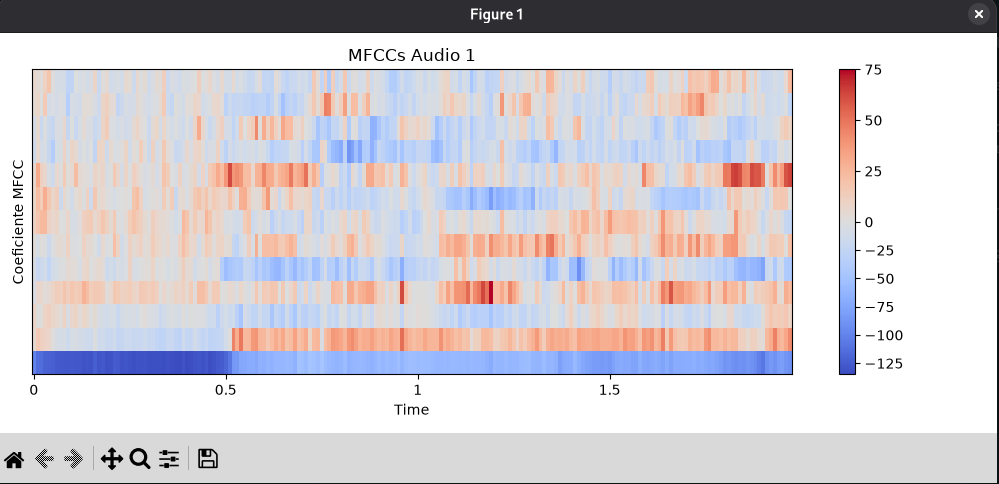
\includegraphics[width=\linewidth]{img1.png}
		\caption{MFCC Manual - Audio 1 (13 coeficientes).}
		\label{fig:mfcc_manual_1}
	\end{minipage}\hfill
	\begin{minipage}{0.48\textwidth}
		\centering
		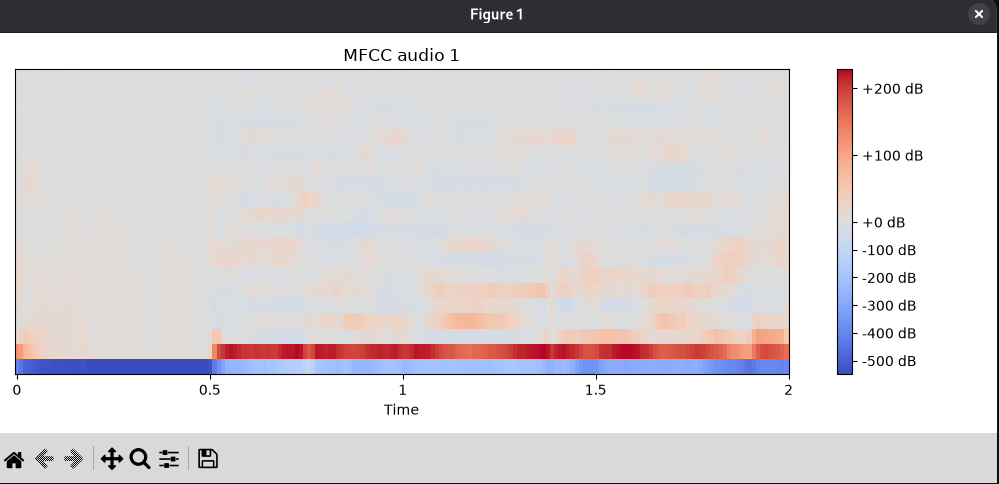
\includegraphics[width=\linewidth]{img2.png}
		\caption{MFCC Librosa - Audio 1 (20 coeficientes).}
		\label{fig:mfcc_librosa_1}
	\end{minipage}
	\caption{Comparación de coeficientes MFCC para el Audio 1.}
	\label{fig:audio1_comp}
\end{figure}

\subsubsection{Análisis de resultados y diferencias observadas}
\begin{itemize}
	\item \textbf{Estructura Temporal:} En la implementación manual se aprecian claramente dos etapas: un intervalo de silencio inicial de $0$ a $0.5\,\text{s}$ caracterizado por coeficientes base fuertemente negativos ($\approx -125$), seguido de la actividad acústica de la palabra \textit{«Casa»} a partir de $t = 0.52\,\text{s}$. En Librosa, el silencio inicial se sitúa en magnitudes en torno a $-500\,\text{dB}$ y la zona fonética eleva su energía por encima de $+200\,\text{dB}$.
	\item \textbf{Resolución y Contraste Cepstral:} La versión manual ofrece una discriminación visual más detallada en los coeficientes intermedios y superiores (órdenes 2 a 12), producto del \textit{liftering} sinusoidal que balancea las amplitudes relativas. Por el contrario, en Librosa la escala está dominada casi en su totalidad por el coeficiente de orden cero ($c_0$), el cual encapsula la energía logarítmica total de la trama y comprime la variación visual de los coeficientes de orden mayor.
	\item \textbf{Tiempos de Ejecución:} La ejecución manual para este audio tomó aproximadamente $0.308\,\text{s}$, mientras que Librosa requirió $1.171\,\text{s}$. Esta diferencia inicial responde al tiempo de carga e importación diferida de módulos y caché de filtros que efectúa Librosa en su primera invocación.
\end{itemize}

\subsection{Comparación del segundo audio (Audio 2: «La casa es grande»)}
La Figura~\ref{fig:audio2_comp} expone los coeficientes MFCC correspondientes a la frase en habla continua.

\begin{figure}[H]
	\centering
	\begin{minipage}{0.48\textwidth}
		\centering
		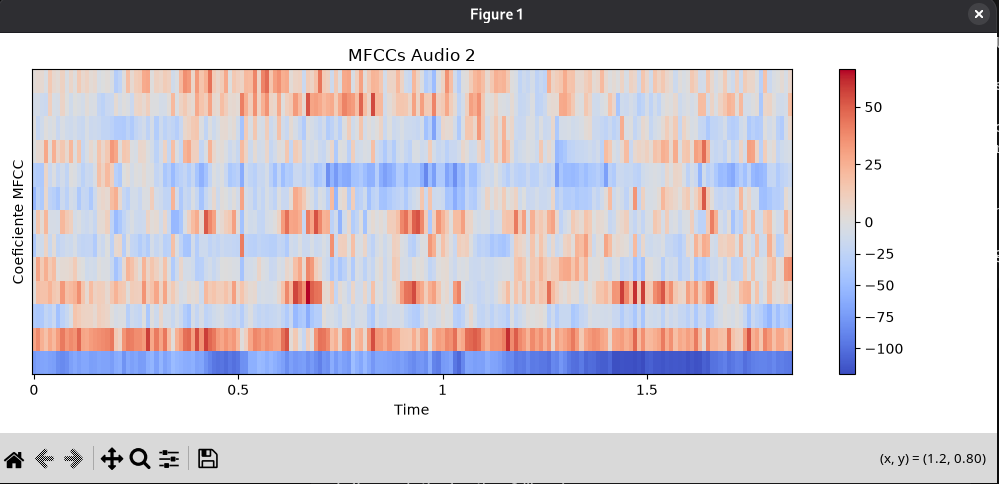
\includegraphics[width=\linewidth]{img3.png}
		\caption{MFCC Manual - Audio 2 (13 coeficientes).}
		\label{fig:mfcc_manual_2}
	\end{minipage}\hfill
	\begin{minipage}{0.48\textwidth}
		\centering
		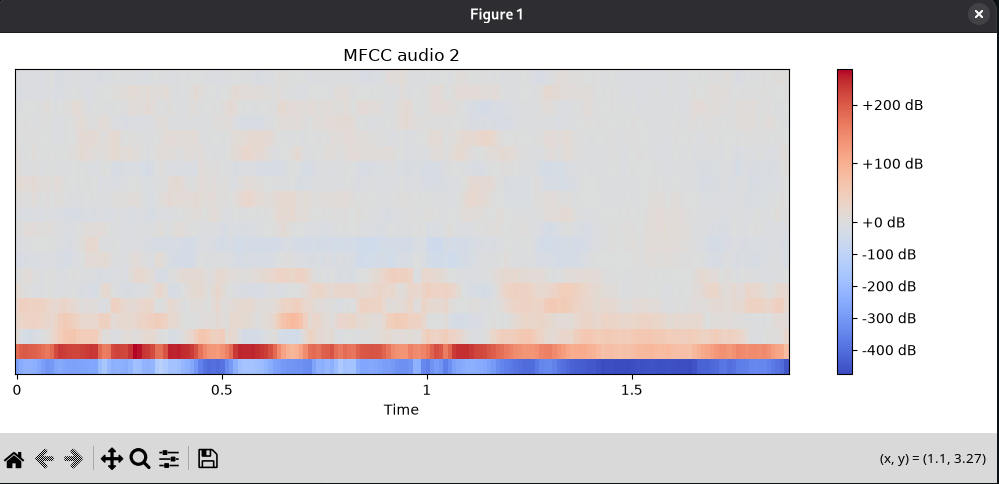
\includegraphics[width=\linewidth]{img4.png}
		\caption{MFCC Librosa - Audio 2 (20 coeficientes).}
		\label{fig:mfcc_librosa_2}
	\end{minipage}
	\caption{Comparación de coeficientes MFCC para el Audio 2.}
	\label{fig:audio2_comp}
\end{figure}

\subsubsection{Análisis de resultados y diferencias observadas}
\begin{itemize}
	\item \textbf{Articulación Continua:} En el Audio 2 la actividad fonética se extiende a lo largo de toda la ventana temporal ($0$ a $1.85\,\text{s}$). En la matriz manual se diferencian con nitidez los formantes y transiciones consonántico-vocálicas asociadas a las sílabas constitutivas de la frase.
	\item \textbf{Discrepancia en Magnitudes y Rango Dinámico:} En la gráfica de Librosa la barra de color muestra un rango dinámico extremo (de $-400\,\text{dB}$ a $+250\,\text{dB}$), lo cual satura visualmente los coeficientes superiores dejándolos con un tinte homogéneo y tenue. En el cálculo manual, el rango oscila entre $-100$ y $+70$, permitiendo apreciar el contorno de la envolvente espectral en todos los órdenes.
	\item \textbf{Tiempos de Cómputo en Régimen Estable:} Una vez inicializados los módulos internos en la memoria del intérprete, el cálculo de Librosa para el segundo audio descendió a $0.049\,\text{s}$, mientras que la versión manual optimizada con \texttt{np.lib.stride\_tricks} y multiplicación matricial requirió únicamente $0.024\,\text{s}$, demostrando una alta eficiencia computacional al evitar la sobrecarga de generalización que maneja la librería.
\end{itemize}



\newpage

\section{Conclusiones}
A través de la presente práctica se implementó y validó exitosamente la cadena matemática para la extracción de coeficientes MFCC, contrastando un modelo manual frente a la biblioteca especializada Librosa. Se concluye que:
\begin{itemize}
	\item \textbf{Causas de variación espectral:} Las discrepancias visuales y cuantitativas entre ambos métodos obedecen a decisiones de preprocesamiento y diseño espectral:
	\begin{enumerate}
		\item \textit{Preénfasis:} La implementación manual incorpora un filtro FIR ($\alpha = 0.97$) que resalta componentes de alta frecuencia antes del ventaneo; Librosa omite esta etapa por defecto.
		\item \textit{Fórmula Mel y Banco de Filtros:} La implementación manual emplea la fórmula estándar de O'Shaughnessy ($2595\log_{10}$) con triángulos sin normalizar en área, mientras que Librosa implementa por defecto el banco de Slaney (\texttt{htk=False, norm='slaney'}), escalando cada filtro por su ancho de banda efectivo.
		\item \textit{Compresión Dinámica:} El uso de \texttt{power\_to\_db} en Librosa frente al simple logaritmo neperiano (\texttt{np.log}) en el desarrollo manual genera escalas de amplitud dispares.
		\item \textit{Liftering:} La inclusión del filtro sinusoidal en la versión manual equilibra las amplitudes relativas de los coeficientes $c_1$ a $c_{12}$, contrarrestando el dominio abrumador del coeficiente de energía $c_0$, efecto ausente en la salida estándar de Librosa.
	\end{enumerate}
	\item \textbf{Eficiencia Computacional:} El cómputo manual vectorizado evidenció un rendimiento sumamente competitivo ($0.024\,\text{s}$ frente a $0.049\,\text{s}$ en régimen estable), confirmando que una implementación compacta en NumPy/SciPy sin dependencias de alto nivel resulta viable y eficiente para sistemas de reconocimiento de patrones y habla embebidos o en tiempo real.
\end{itemize}

\newpage


\begin{thebibliography}{99}

	\bibitem{librosa_scipy} 
	B.~McFee, C.~Raffel, D.~Liang, D.~P.~W.~Ellis, M.~McVicar, E.~Battenberg y O.~Nieto, ``librosa: Audio and Music Signal Analysis in Python,'' en \textit{Proceedings of the 14th Python in Science Conference (SciPy 2015)}, Austin, TX, USA, 2015, pp. 18--25. doi: 10.25080/Majora-7b98e3ed-003.
	
	\bibitem{davis_mermelstein} 
	S.~Davis y P.~Mermelstein, ``Comparison of parametric representations for monosyllabic word recognition in continuously spoken sentences,'' \textit{IEEE Transactions on Acoustics, Speech, and Signal Processing}, vol. 28, no. 4, pp. 357--366, ago. 1980. doi: 10.1109/TASSP.1980.1163420.
	
	\bibitem{rabiner_juang} 
	L.~Rabiner y B.~H.~Juang, \textit{Fundamentals of Speech Recognition}. Englewood Cliffs, NJ, USA: Prentice Hall, 1993.
	
	\bibitem{huang_spokentext} 
	X.~Huang, A.~Acero y H.-W.~Hon, \textit{Spoken Language Processing: A Guide to Theory, Algorithm, and System Development}. Upper Saddle River, NJ, USA: Prentice Hall PTR, 2001.
\end{thebibliography}
	
\end{document}